% chapter08.tex

 %%%%%%%%%%%%%%%%%%%%%%%%%%%%%%%%%%%%%%%%%%%%%%%%%%%%%%%%%%%%%%%%%%%%%%%%%%%%%
 %                                                                           %
 %    PyMS documentation                                                     %
 %    Copyright (C) 2005-2010 Vladimir Likic                                 %
 %                                                                           %
 %    The files in this directory provided under the Creative Commons        %
 %    Attribution-NonCommercial-NoDerivs 2.1 Australia license               %
 %    http://creativecommons.org/licenses/by-nc-nd/2.1/au/                   %
 %    See the file license.txt                                               %
 %                                                                           %
 %%%%%%%%%%%%%%%%%%%%%%%%%%%%%%%%%%%%%%%%%%%%%%%%%%%%%%%%%%%%%%%%%%%%%%%%%%%%%

\chapter{Labelled data related algorithms}


\section
{Mass Isotopomer Distribution Extraction in $^{13}$C Experiments}

\noindent
[ \emph{This example is in pyms-test/91} ]

The aim of this method is to semi-automatically extract the isotopomer mass
distribution (MID) of each metabolite of interest from raw GC-MS data files.

A metabolite with n carbon atoms can be labelled at any position resulting in
2$^{n}$ different combinations, which are called isotopomers. For example, 
if a metabolite contains three carbon atoms and we denote unlabelled atom with
 ‘0’ and labelled with ‘1’, the possible labelling patterns for the carbon 
backbone are 000, 001, 010, 011, 100, 101, 110, 111. Mass spectrometry can only
resolve isotopomer distribution completely if enough fragments can be detected 
(for a compound with n carbon atoms this means 2$^{n}$ – 1 different fragments 
containing different number and/or combinations of carbons).

The same metabolite has n+1 different masses: base mass M (000), singly labelled
mass M+1 (001, 010, 100), doubly labelled mass M+2 (011, 101, 110) and fully 
labelled mass M+3 (111). The MS measurement of the molecular ion gives the mass 
isotopomer distribution (e.g. M, M+1, M+2, M+3) of the compound.

The algorithm developed ( Figure \ref{fig:pymsMIDs}) relies on the value of the metabolite’s diagnostic
fragment ion to extract the ion chromatograms from the data file.
Metabolite’s retention time is then used for the feature extraction. Peak
apex is defined as the local maximum within a specified window of the given
retention time. Left and right boundaries are defined as the first local minima on
the left and right of the peak apex. The extraction of left and right boundary
values is repeated for the characteristic fragment ion and its subsequent
isotopomers.

\begin{figure}
  \begin{center}
    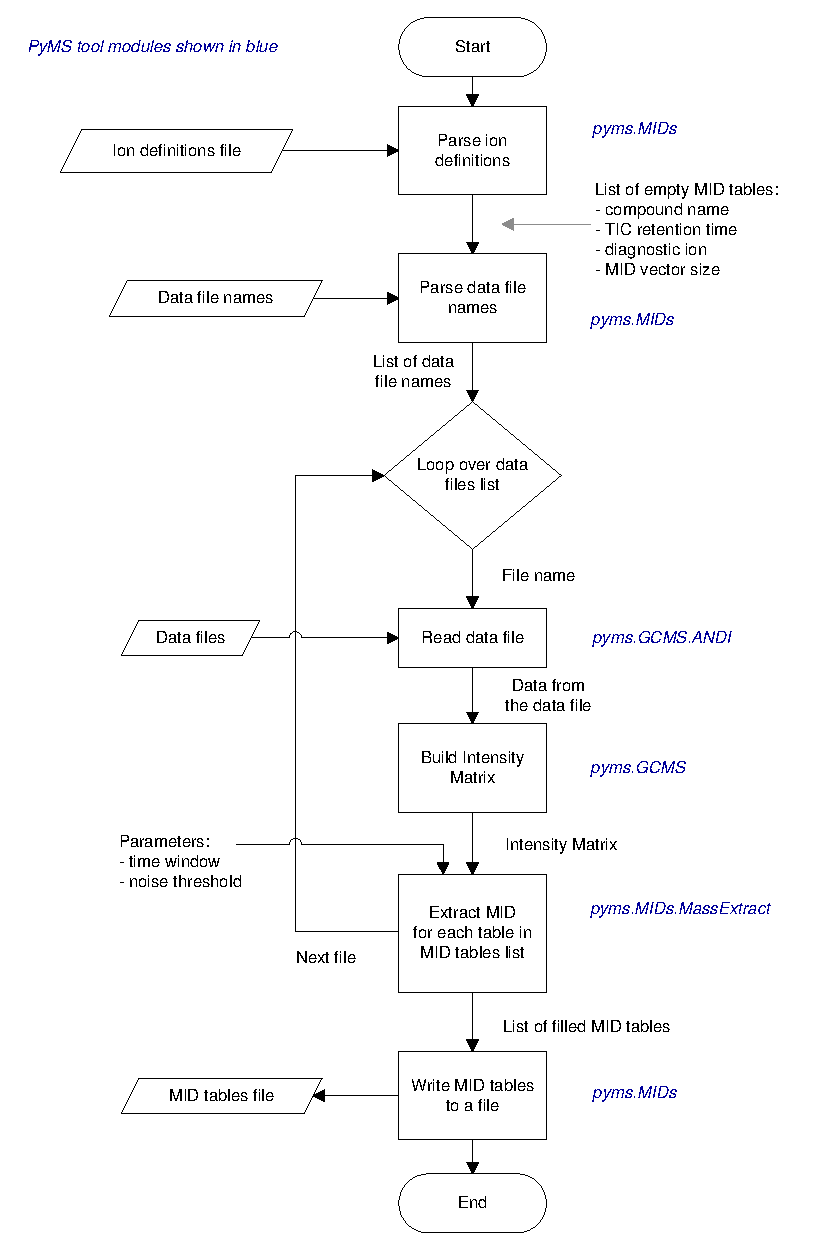
\includegraphics[scale=0.33]{graphics/chapter08/pymsMIDs.eps}
  \end{center}
  \caption{Data Flow Chart}
  \label{fig:pymsMIDs}
\end{figure}

The boundary values are then averaged for each file and the overall isotopomer
intensity is quantified by summing all of the intensities between average left and
right boundary values inside each ion chromatogram. The results are
then normalised to obtain mass isotopomer distribution (i.e. percentage
contributions of M, M+1, M+2, M+3, etc. ions). Where M represents the base mass of 
a non-labelled ion, M+1 represents the ion incorporating a single labelled atom, 
M+2 ion is the one with two labelled atoms, etc.

In the example, experimental data are saved as a series of .CDF files, and the base 
file name is:
\begin{verbatim}
 '/home/projects/PyMS/data-0903/a0903_'
\end{verbatim}
 with the extension file numbers '297, 298, 299'. The compound is Alanine, the 
retention time is 411 seconds and the diagnostic ion is 190 with MID size of 6 
(i.e. ions to be extracted are 190, 191, 192, 193, 194, and 195). Window size 
used is 4 seconds.

To enter the above input data:

\begin{verbatim}
>>> file_base = '/home/projects/PyMS/data-0903/a0903_'
>>> file_numbers = (297, 298, 299)
>>> compound = 'Alanine'
>>> ion = 190
>>> rt = 411 
\end{verbatim}

and to enter the parameters:

\begin{verbatim} 
>>> mid_size = 6 
>>> win_size = 4 
\end{verbatim}

Finally, to extract MID:
\begin{verbatim}
>>> import pyms.LabelledData.MID.Extract.Function
>>> extract_mid(file_base, file_numbers, compound, ion, rt, mid_size, win_size)

This will give the following result:

\begin{verbatim}
Alanine
 -> Reading netCDF file '/home/projects/PyMS/data-0903/a0903_297.CDF'
Mass Isotopomer Distribution (MID): 615040.0 128760.0 58418.0 8837.0 1440.0 0.0 

 -> Reading netCDF file '/home/projects/PyMS/data-0903/a0903_298.CDF'
Mass Isotopomer Distribution (MID): 738048.0 155456.0 68656.0 9833.0 1859.0 0.0 

 -> Reading netCDF file '/home/projects/PyMS/data-0903/a0903_299.CDF'
Mass Isotopomer Distribution (MID): 982400.0 207456.0 85200.0 12021.0 3368.0 908.0 
\end{verbatim}


\section
{Mass Isotopomer Distribution Correction in $^{13}$C Experiments}

\noindent
[ \emph{This example is in pyms-test/92} ]

Method implemented is that of Wittman and Heinzle \cite{wittman99}, and the details
of the example are given in Nanchen et al \cite{nanchen07}. 

Higher mass ion intensities (M, M + 1, M + 2, etc.) from $^{13}$C tracer 
experiments will include natural abundance of non-C isotopes and also natural 
abundance of $^{13}$C isotopes inside the GC-MS derivatization reagent, if 
applicable. The function takes the experimental ion intensities, which are obtained 
prior via integration of individual ion chromatograms, calculates the corresponding 
mass distribution vector and performs the correction  for natural isotope 
abundances of C, O, N, H, Si, and S atoms, as well as any unlabelled biomass (this 
corrects for the fact that in practice substrate is never 100\%\ labelled). The 
result is a corrected mass distribution vector. Fractional labelling value is also
provided as a check, and it should be equal to the fractional labelling of the
input substrate.

Experimental data is entered using the 'mdv' variable. In the example of
alanine fragment (M-57)+ \cite{nanchen07} there are n = 3 exogenous (non-natural
abundance) C atoms, and the length of the mass distribution vector
is chosen to be n+1=4. Hence only first four intensities (ion counts)
from the mass spectrum, corresponding to M, M+1, M+2 and M+3, are entered.

\begin{verbatim}
>>> mdv = [737537, 179694, 88657, 178433]
>>> n = len(mdv) - 1
\end{verbatim}

Determine the number of C, O, N, H, Si, and S atoms in the fragment,
noting that the number of C atoms excludes C atoms which may contain
exogenous $^{13}$C atoms. For the alanine (M-57)+ fragment these
numbers are C=8, O=2, N=1, H=26, Si=2, and S=0.

\begin{verbatim} 
>>> atoms = { 'c':8, 'o':2, 'n':1, 'h':26, 'si':2, 's':0}
\end{verbatim}

Import the relevant modules:

\begin{verbatim}
>>> import numpy
>>> import pyms.LabelledData.MID.Correct.Function
>>> import pyms.LabelledData.MID.Correct.Constants
\end{verbatim}

Calculate the overall correction matrix:

\begin{verbatim}
>>> c_corr = pyms.LabelledData.MID.Correct.Function.overall_correction_matrix(n, mdv, atoms)

Calculating c correction matrix

Calculating h correction matrix

Calculating si correction matrix

Calculating o correction matrix

Calculating n correction matrix

Calculating s correction matrix

Calculated overall correction matrix.

>>> c_corr array([[0.77152972 , 0.         , 0.         , 0.        ],
                  [0.1508547  , 0.77152972 , 0.         , 0.        ],
                  [0.06721399 , 0.1508547  , 0.77152972 , 0.        ],
                  [0.00866575 , 0.06721399 , 0.1508547  , 0.77152972]])
\end{verbatim}

Calculate the exclusive mass isotope distribution of the carbon skeleton:

\begin{verbatim}
>>> mdv_alpha_star = pyms.LabelledData.MID.Correct.Function.c_mass_isotope_distr(mdv, c_corr)
>>> mdv_alpha_star array([[ 0.7729932 ],
                          [ 0.03719172],
                          [ 0.01830562],
                          [ 0.17150946]])
\end{verbatim}

Correct for unlabelled biomass. This example accounts for the contribution
of 1\%\ unlabelled biomass.

\begin{verbatim}
>>> f_unlablelled = 0.01 
>>> mdv_aa = pyms.LabelledData.MID.Correct.Function.corr_unlabelled(n, mdv_alpha_star, f_unlabelled)
>>> mdv_aa array([[ 0.77102099],
                  [ 0.03725005],
                  [ 0.01848709],
                  [ 0.17324187]])
\end{verbatim}

Calculate the fractional labelling:

\begin{verbatim}
>>> fl = pyms.LabelledData.MID.Correct.Function.fract_labelling(n, mdv_aa)
Fractional labelling FL: 0.197983278219
\end{verbatim}
